\documentclass[letterpaper,11pt,oneside,reqno]{article}

%%%%%%%%%%%%%%%%%%%%%%%%%%%%%%%%%%%%%%%%%%%%%%%%%%%%%%%%%%%%

\usepackage[pdftex,backref=page,colorlinks=true,linkcolor=blue,citecolor=red]{hyperref}
\usepackage[alphabetic,nobysame]{amsrefs}

%%%%%%%%%%%%%%%%%%%%%%%%%%%%%%%%%%%%%%%%%%%%%%%%%%%%%%%%%%%%
%main packages
\usepackage{amsmath,amssymb,amsthm,amsfonts,mathtools}
\usepackage{graphicx,color}
\usepackage{upgreek}
\usepackage[mathscr]{euscript}

%equations
\allowdisplaybreaks
\numberwithin{equation}{section}

%tikz
\usepackage{tikz}
\usetikzlibrary{shapes,arrows,positioning,decorations.markings}

%conveniences
\usepackage{array}
\usepackage{adjustbox}
\usepackage{cleveref}
\usepackage{enumerate}
\usepackage[all,cmtip]{xy}

%paper geometry
\usepackage[DIV=12]{typearea}

%%%%%%%%%%%%%%%%%%%%%%%%%%%%%%%%%%%%%%%%%%%%%%%%%%%%%%%%%%%%
%draft-specific
\synctex=1
% \usepackage{refcheck,comment}

%%%%%%%%%%%%%%%%%%%%%%%%%%%%%%%%%%%%%%%%%%%%%%%%%%%%%%%%%%%%
%this paper specific
\newcommand{\ssp}{\hspace{1pt}}

%%%%%%%%%%%%%%%%%%%%%%%%%%%%%%%%%%%%%%%%%%%%%%%%%%%%%%%%%%%%
\newtheorem{proposition}{Proposition}[section]
\newtheorem{lemma}[proposition]{Lemma}
\newtheorem{corollary}[proposition]{Corollary}
\newtheorem{theorem}[proposition]{Theorem}
%%%%%%%%%%%%%%%%%%%%%%%%%%%%%%%%%%%%%%%%%%%%%%%%%%%%%%%%%%%%
\theoremstyle{definition}
\newtheorem{definition}[proposition]{Definition}
\newtheorem{remark}[proposition]{Remark}
%%%%%%%%%%%%%%%%%%%%%%%%%%%%%%%%%%%%%%%%%%%%%%%%%%%%%%%%%%%%

\begin{document}
\title{Random Fibonacci Words}

% OTHER AUTHORS

\author{Leonid Petrov; based on the joint work with Jeanne Scott \cite{PetrovScott2024Fibonacci}}

\date{Talk at University of Illinois at Urbana-Champaign, Integrability \& Representation Theory (IRT) Seminar, February 20, 2025}


\maketitle

\begin{abstract}
	Fibonacci words are words of 1's and 2's, graded by the total sum of the digits. They form a differential poset ($\mathbb{YF}$) which is an estranged cousin of the Young lattice powering irreducible representations of the symmetric group. We introduce families of "coherent" measures on $\mathbb{YF}$ depending on many parameters, which come from the theory of clone Schur functions \cite{okada1994algebras}. We characterize parameter sequences ensuring positivity of the measures, and we describe the large-scale behavior of some ensembles of random Fibonacci words. The subject has connections to total positivity of tridiagonal matrices, Stieltjes moment sequences, orthogonal polynomials from the (q-)Askey scheme, and residual allocation (stick-breaking) models.
\end{abstract}

\section*{What is this text}

These are notes for a chalk talk, prepared based on the paper
\cite{PetrovScott2024Fibonacci}, in the ``extended lecture notes''
style, similar to my \href{https://lpetrov.cc/rmt25/}{random matrix course}.
Along the notes, there are numerous skipped details,
which are left as exercises for the reader.

\setcounter{tocdepth}{1}
\tableofcontents
\setcounter{tocdepth}{3}

\section{Motivation 1. De Finetti's theorem and Pascal triangle}

\subsection{}

\begin{definition}
	A sequence $X_1,X_2,\ldots $
	of binary random variables
	(taking values in $\{0,1\}$)
	is called \emph{exchangeable}
	if for any $n$ and any permutation $\sigma$ of $\{1,2,\ldots,n\}$ the joint distribution of $X_1,X_2,\ldots,X_n$ is the same as the joint distribution of $X_{\sigma(1)},X_{\sigma(2)},\ldots,X_{\sigma(n)}$.
\end{definition}

Exchangeable sequences are more than just Bernoulli iid sequences with some
parameter $p\in[0,1]$. Consider the Polya urn scheme.

Start with an urn containing $b$ black and $w$ white balls.
At each step, draw a ball uniformly at random from the urn
and put it back along with another ball of the same color.

The sequence of ball colors drawn from the urn is exchangeable.

At time $n$, there are $n$ new balls in the urn, and the distribution of the number of, say,
black balls,
\begin{equation*}
	\operatorname{\mathbb{P}}\left( \textnormal{black}=k \right) = M_n(k),
	\qquad k=0,1,\ldots,n,
\end{equation*}
is called the ($n$-th) \emph{coherent measure}.
We can talk about $S_n$, the random variable which is the number of black balls drawn by time $n$.
The coherent measures $M_n$ for various $n$ satisfy certain linear
recurrence relations.

One can convince oneself that the space of coherent measures is
the same as the space of exchangeable random sequences of 0's and 1's.
This space is a convex set, moreover, it is a simplex.

\begin{definition}
	A point $A$ in a convex linear set is called
	\emph{extremal} if it cannot be written as a convex combination of other points in the set.
	A simplex is a convex set in which every point is a unique
	convex combination of extremal points.

	Examples: triangle vs square vs disc.
\end{definition}

Extreme points of the simplex corresponding to the Pascal triangle
are given by iid sequences,
that is, Bernoulli product measures on $\left\{ 0,1 \right\}^\infty$.
This is de Finetti's theorem.

\subsection{}

Coherent measures on Pascal triangle are related to exchangeable
sequences of 0's and 1's. The \emph{boundary} of the Pascal
triangle encodes all possible coherent measures via the law of large numbers,
\begin{equation*}
	\frac{S_n}{n}\to \mu \quad \textnormal{on} \quad [0,1].
\end{equation*}
Extreme measures correspond to delta point masses.
For example, the Polya urn for $a=b=1$ corresponds to $\mu$ being the
uniform measure on $[0,1]$.

\subsection{Lonely paths}

There are two distinguished paths in the Pascal triangle, the
\emph{lonely paths} $0\to00\to000\to\ldots $
and
$1\to 11\to111\to\ldots $, which are characterized by the
property that \cite{KerovGoodman1997}
\begin{quote}
	All but finitely many vertices in the path have a single immediate predecessor.
\end{quote}
These paths correspond to the extreme measures
with $\mu=\delta_0$ and $\mu=\delta_1$, respectively.

It turns out that all other extreme measures on the Pascal triangle
are obtained by a \emph{``convex interpolation'' of these two lonely path measures}.
Note that this interpolation is \emph{not} the same as the convex combination
of coherent measures, so the points $p\in(0,1)$ are still extremal
for the space of coherent measures. However, the boundary
of the Pascal triangle clearly contains the linear
piece between $\delta_0$ and $\delta_1$.


\section{Motivation 2. Young lattice}

The Young lattice $\mathbb{Y}$ of integer partitions ordered
by the relation ``adding a box''
encodes another meaningful structure --- irreducible representations of the symmetric groups.
The boundary encodes the irreducible representations of the infinite symmetric group $S(\infty)$.

\subsection{}
The Young lattice is a \emph{differential poset} \cite{stanley1988differential},
\cite{fomin1994duality},
in the sense that
\begin{quote}
	for each $\lambda$, there is one more element in the set
	$\left\{ \nu\colon\nu=\lambda+\square \right\}$ than
	in the set $\left\{ \mu\colon\mu=\lambda-\square \right\}$.
\end{quote}
Differential poset
property implies that
for $f^\lambda$ the number of paths from $\varnothing$ to $\lambda$, we have
\begin{equation*}
	\sum_{|\lambda|=n}(f^\lambda)^2=n!, \qquad \textnormal{define}\qquad
	M_n(\lambda)\coloneqq\frac{(f^\lambda)^2}{n!}.
\end{equation*}
The measure $M_n$ is called \emph{Plancherel}, it is coherent
and extremal. It corresponds to the regular representation of $S(\infty)$,
which is irreducible.

\subsection{}

There are two lonely paths here, as well --- corresponding to growing
one-row and one-column partitions.

\subsection{}

All extreme coherent measures on the Young lattice are given by specializations
of Schur symmetric functions, and have the form
\begin{equation*}
	M_n(\lambda)=s_\lambda(\vec \alpha;\vec \beta;\gamma)\cdot f^\lambda.
\end{equation*}
The problem of describing the boundary of $\mathbb{Y}$ is equivalent to
the problem of finding parameters $\vec \alpha,\vec \beta,\gamma$ such that
the Schur functions $s_\lambda(\vec \alpha;\vec \beta;\gamma)$ are nonnegative
for all $\lambda$.

Schur functions are (essentially) determinants, and
for the Young lattice, we have a great match between these multiparameter functions and
extreme coherent measures.
The algebraic combinatorial property of the Schur
polynomials which connects them to the Young lattice
is the Pieri rule:
\begin{equation*}
	p_1 s_\lambda=\sum_{\nu\colon \nu=\lambda+\square}s_\nu.
\end{equation*}

\begin{remark}
	The parameters $\vec \alpha;\vec \beta;\gamma$ encode the law of large
	numbers for the growing random Young diagram.
	The parameters $\alpha_i$ and $\beta_i$ are the lengths of the $i$-th row and column
	scaled by $n^{-1}$,
	and $\gamma$ is the scaled excess $1-\sum(\alpha_i+\beta_i)$. For
	the Plancherel measure, rows and columns grow as $\sqrt n$,
	so $\alpha_i=\beta_i=0$ and $\gamma=1$.
\end{remark}


\section{Another differential poset --- the Young--Fibonacci lattice}

\subsection{}

A natural question arises: do other differential posets exist?
Indeed, there exists another fundamental example, denoted $\mathbb{YF}$, which, upon first examination,
might seem contrived and unnatural.
(While there also
exists a family of posets interpolating between
$\mathbb{YF}$ and $\mathbb{Y}$, we shall not explore that
here.)

\subsection{}

The Young--Fibonacci lattice $\mathbb{YF}$
can be formed starting from the single edge $\varnothing\to 1$,
by successive reflection. We then encode the new vertices as starting from $1$ (followed by the
old vertex index from the level $n-1$), and the
reflected vertices as starting from $2$ (followed by the
old vertex index from the level $n-2$).

\begin{figure}[htp]
	\centering
	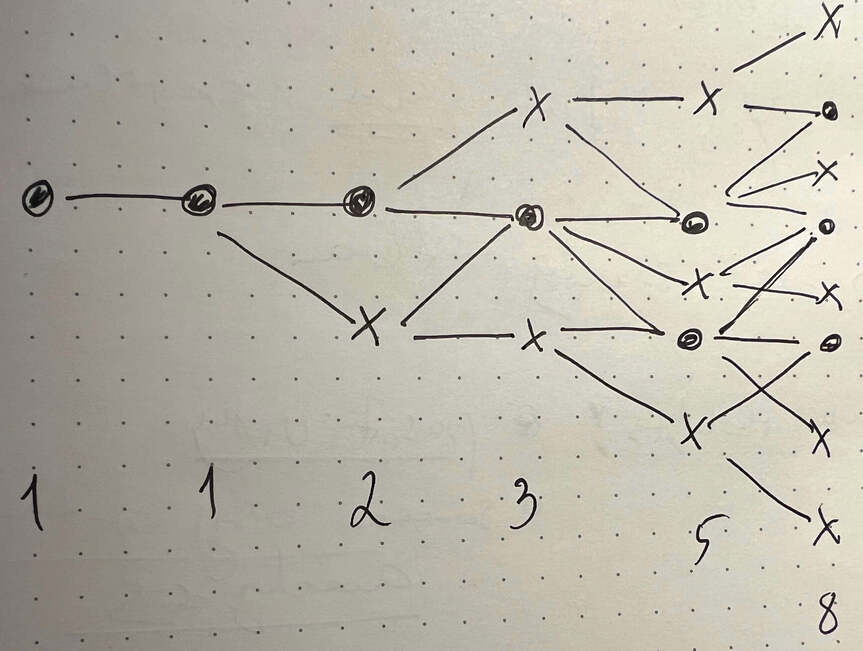
\includegraphics[width=0.5\textwidth]{YF}
\end{figure}

\subsection{}

$\mathbb{YF}$ is a graded poset formed
by Fibonacci words (binary words whose digits lie in
$\{1,2\}$), graded by the sum of their digits.

We denote the set of all Fibonacci words of weight $n$ by
$\mathbb{YF}_n$. Clearly, the total number of such words is
the $n$th Fibonacci number (with $F_0 = F_1 = 1$). The poset
$\mathbb{YF}$ is then the disjoint union of all
$\mathbb{YF}_n$ for $n = 0,1,2,\ldots,$ with rank function
given by the weight $|w| = n$. We always identify the empty
word $\varnothing$ with $\mathbb{YF}_0$.

\begin{definition}[Young--Fibonacci Partial Order]
\label{def:YF-partial-order}
We say a Fibonacci word $w$ \emph{covers} another Fibonacci word $v$ if $|v| = |w| - 1$ and one can transform $w$ to $v$ by one of the following rules:
\begin{enumerate}
\item If $w = 1 \,v$, then we delete the leftmost $1$ to obtain $v$.
\item If $w = 2 \,u$ for some $u$, then we obtain $v$ by turning the leftmost $2$ into a $1$ or by removing the leftmost inserted $1$ after a $2$.
\end{enumerate}
\end{definition}

\begin{figure}[htpb]
	\centering
	\begin{equation*}
		\xymatrixrowsep{0.3in}
		\xymatrixcolsep{0.15in}
		\xymatrix{ \varnothing \ar@{-}[d] & & & & & & &  \\
		1 \ar@{-}[d] \ar@{-}[drrrrrrr] & & & & & & & \\
		11  \ar@{-}[d] \ar@{-}[drrrr] & & & & & & & 2  \ar@{-}[d] \ar@{-}[dlll] \\
		111  \ar@{-}[d] \ar@{-}[drr] & & & & 21 \ar@{-}[d] \ar@{-}[dll] \ar@{-}[dr] & & & 12  \ar@{-}[d] \ar@{-}[dll] \\
		1111  \ar@{-}[d] \ar@{-}[dr]  & &211  \ar@{-}[d] \ar@{-}[dl] \ar@{-}[dr] & &121 \ar@{-}[d] \ar@{-}[dl]  &22 \ar@{-}[d] \ar@{-}[dll]|\hole \ar@{-}[dr]
		& &112  \ar@{-}[d] \ar@{-}[dl]  \\
		11111 & 2111 & 1211 & 221 & 1121 & 122 & 212 & 1112 }
	\end{equation*}
	\caption{The Young--Fibonacci lattice up to level $n=5$.}
	\label{fig:YF_lattice}
\end{figure}

\subsection{}

The Young--Fibonacci lattice is a differential poset. Hence, we have
\begin{equation*}
	\sum_{|w|=n}(\dim w)^2=n!,
\end{equation*}
and we can define the \emph{Plancherel measure}
\begin{equation*}
	M_n(w)\coloneqq \frac{(\dim w)^2}{n!}.
\end{equation*}
Note that the $\mathbb{YF}$-dimension is very
different from the Young lattice one.
For $w \in \mathbb{YF}_n$ of the form
$w = a_1 \, a_2 \cdots a_\ell$, we have
\[
\dim(w)
\;=\;
\prod_{\substack{1 \,\leq\, j \,\leq\, \ell \\ a_j \,=\, 2}}
\bigl( |u_j| + 1 \bigr),
\]
where $u_j$ is the subword to the right of the $j$-th digit.

The Plancherel measure is extremal.

\subsection{Boundary problem}

We would like to understand the boundary of $\mathbb{YF}$.
As in the Young and Pascal cases, the boundary should capture the law of
large numbers for the growing Fibonacci words.

\subsection{Lonely paths}

In contrast with the Young lattice and the Pascal triangle,
the Young--Fibonacci lattice has many lonely paths.
Namely, there is a lonely path from each Fibonacci word $w$:
\begin{equation*}
	1w, \quad 11w, \quad 111w, \quad \ldots
\end{equation*}
We denote it by $1^\infty w$.
Lonely paths correspond to extreme measures,
so the boundary has a ``discrete component''
$1^\infty\mathbb{YF}$.

The full boundary looks as the Plancherel point,
connected to all points $1^\infty w$, $w\in\mathbb{YF}$,
by linear segments (via the ``convex interpolation'' as in the
Pascal case --- recall that these segments are still extremal
for coherent measures).
Graphically, the boundary is a ``star'' with the Plancherel point
in the center.

\subsection{Boundary description --- references}

The boundary of the Young--Fibonacci lattice
was established in the following works:
\begin{itemize}
	\item \cite{KerovGoodman1997} described the Martin
		boundary, which is the set of all coherent measures
		obtained by finite rank approximation. It remained an
		open problem to show that this list is of extreme measures.
	\item \cite{gnedin2000plancherel}, shown that the Plancherel measure is extremal
		(ergodic), by considering the scaling limit of
		Plancherel random Fibonacci words. They essentially show that this limit is incompatible
		with any other possible point from the Martin boundary, thus
		leading to the extremality.
	\item Preprints
		\cite{BochkovEvtushevsky2020},
		\cite{Evtushevsky2020PartII}
		established the full boundary description by showing
		the extremality (ergodicity) of all coherent measures.
\end{itemize}

\subsection{How about Schur functions?}

While we now understand the boundary's structure, a natural question arises: are there
elegant functions, analogous to determinantal Schur functions, that capture the
combinatorial properties of this lattice? Indeed, such functions exist - the
\emph{clone Schur functions} introduced by Okada \cite{okada1994algebras}. These
functions were specifically developed to provide an algebraic framework for the
Young--Fibonacci lattice, paralleling how classical Schur functions encode the
structure of the Young lattice.

The clone Schur functions $s_w(\vec x\mid \vec y)$
(definition later)
satisfy a Pieri rule:
\begin{equation*}
	x_{|w|+1}s_w(\vec x\mid \vec y)=\sum_{v\colon v\nearrow w}s_v(\vec x\mid \vec y).
\end{equation*}
There are \emph{clone coherent measures} defined from clone Schur functions,
\begin{equation*}
	M_n(w)=s_w(\vec \alpha;\vec \beta;\gamma)\cdot \dim w,
\end{equation*}
but \textbf{they are not extremal} (except for the Plancherel case).

\subsection{Now, briefly, what we do with this}

We get the following main results:
\begin{enumerate}
	\item Complete classification of 
		clone coherent measures which are positive. 
		This is related to total positivity of tridiagonal matrices and Stieltjes moment
		problems.
		In fact, we obtain a new, narrower notion of tridiagonal
		positivity called \emph{Fibonacci positivity}. 
	\item We describe a number of examples of Fibonacci positive specializations.
	\item For several Fibonacci positive specializations, we consider the large-scale behavior of random Fibonacci words.
\end{enumerate}

\section{Clone Schur functions and positivity}

\subsection{Definition}

Let $\vec x=(x_1,x_2,\ldots )$ and $\vec y=(y_1,y_2,\ldots)$ be two families of indeterminates.
Define two sequences of tridiagonal determinants as follows:
\begin{equation}
	\label{eq:A_B_dets}
	A_\ell (\vec{x} \mid \vec{y}\ssp) \coloneqq
	\det
	\underbrace{\begin{pmatrix}
	x_1 & y_1 & 0 & \cdots\\
	1 & x_2 & y_2 &\\
	0 & 1 & x_3  & \\
	\vdots & & & \ddots
	\end{pmatrix}}_{\text{$\ell \times \ell $ tridiagonal matrix}} ,
	\qquad
	B_{\ell -1} (\vec{x} \mid \vec{y}\ssp) \coloneqq
	\det
	\underbrace{\begin{pmatrix}
	y_1 & x_1y_2 & 0 & \cdots\\
	1 & x_3 & y_3 &\\
	0 & 1 & x_4 & \\
	\vdots & & & \ddots
	\end{pmatrix}}_{\text{$\ell \times \ell$ tridiagonal matrix}} .
\end{equation}
Here $\ell\ge0$.
For a sequence $\vec u=(u_1,u_2,\ldots)$,
denote its
\emph{shift} by $\vec u+ \ell = (u_{1+\ell} \, ,u_{2+\ell} \, ,\ldots)$, where $\ell\in \mathbb{Z}_{\ge0}$.


\begin{definition}
	\label{def:clone_Schur}
	For any Fibonacci word $w$,
	define the
	(\emph{biserial})
	\emph{clone Schur function} $s_w(\vec{x} \mid \vec{y}\ssp)$ through the following recurrence:
	\begin{equation}
		\label{eq:clone_Schur_recurrence_def}
		s_w (\vec{x} \mid \vec{y}\ssp)
		\coloneqq
		\begin{cases}
			A_k(\vec{x} \mid \vec{y}\ssp), & \textnormal{if $w=1^{k}$ for some $k\ge 0$},\\
			B_k\bigl( \vec{x}+|u| \mid \vec{y}+|u| \bigr)\cdot s_u (\vec{x} \mid \vec{y}\ssp)
			, & \textnormal{if $w=1^k2u$ for some $k\ge 0$}.
		\end{cases}
	\end{equation}
\end{definition}
Note that these functions are not symmetric in the variables,
and the order in the sequences $(x_1,x_2,\ldots)$ and $(y_1,y_2,\ldots)$ is important.

\subsection{Positivity problem: reduction to tridiagonal matrices}

For the positivity of the functions
$s_w(\vec{x} \mid \vec{y}\ssp)$, it is necessary that the 
infinite
tridiagonal matrix 
\begin{equation}
	\label{eq:tridiagonal_matrix}
	\begin{pmatrix}
	x_1 & y_1 & 0 & \cdots\\
	1 & x_2 & y_2 &\\
	0 & 1 & x_3  & \\
	\vdots & & & \ddots
	\end{pmatrix}
\end{equation}
is totally positive (that is, all its minors that are not
identically zero must be positive).

Total positivity of tridiagonal matrices is a well-known phenomenon
\cite{FominZelevinsky1999}.
We have a stronger requirement than just the total positivity
of \eqref{eq:tridiagonal_matrix} --- we need the total positivity of
another family of matrices, 
\begin{equation*}
		\mathcal{B}_r \big( \, \vec{x} \, \big| \, \vec{y} \, \big) \, \coloneqq \
		\begin{pmatrix}
		y_{r+1} & x_{r+1} y_{r+2} & 0 & \cdots\\
		1 & x_{r+3} & y_{r+3} &\\
		0 & 1 & x_{r+4}  & \\
		\vdots & & & \ddots
	\end{pmatrix},
\end{equation*}
for all $r$. The tridiagonal matrix \eqref{eq:tridiagonal_matrix} is a good starting point,
though: it allows us to reparameterize
\begin{equation*}
	x_k=1+t_{k-1},\qquad y_k=t_k,\qquad t_0=0, \qquad t_j>0, \quad j\ge 1.
\end{equation*}
(There are some obvious renormalizations of the parameters 
$\vec x,\vec y$
which we ignore, and 
focus only on the primary case.)

\subsection{Fibonacci positivity: result}

There are two classes of $\vec t$-sequences for which the
specializations of clone Schur functions are positive.
\begin{theorem}
	All Fibonacci positive sequences
	$(\vec x,\vec{y}\ssp)$
	have the form
	\begin{equation*}
		x_k=c_k\ssp (1+t_{k-1}),\qquad y_k=c_k\ssp c_{k+1}\ssp t_k, \qquad k\ge1,
	\end{equation*}
	where $\vec c$ is an
	arbitrary positive sequence,
	and $\vec t=(t_1,t_2,\ldots )$ (with $t_0=0$, for convenience) is
	a positive real sequence of one of the two types:
	\begin{enumerate}[$\bullet$]
		\item (divergent type)
			The infinite series
			\begin{equation}
				\label{eq:divergent_type_A1}
				1+t_1+t_1t_2+t_1t_2t_3+\ldots
			\end{equation}
			diverges, and
			$t_{m+1}\ge 1+t_m$ for all $m\ge 1$;
		\item (convergent type)
			The series \eqref{eq:divergent_type_A1} converges, and
			\begin{equation*}
				 1+t_{m+3}+t_{m+3}t_{m+4}+
				t_{m+3}t_{m+4}t_{m+5}+\ldots
				\ge
				\frac{t_{m+1}}{t_{m+2}(1+t_m-t_{m+1})}
				,
				\qquad
				\textnormal{for all }
				m\ge0.
			\end{equation*}
	\end{enumerate}
	The sequences $\vec c$ and $\vec t$ are determined by $(\vec x,\vec{y}\ssp)$ uniquely.
\end{theorem}

A divergent type sequence can be written
as 
\begin{equation*}
	t_k=k+\varepsilon_1+\ldots+\varepsilon_k ,
\end{equation*}
where $\varepsilon_j\ge 0$. Then the matrices
\eqref{eq:tridiagonal_matrix} and $\mathcal{B}_r$ 
have all minors either identically zero, 
or element of $\mathbb{Z}[\varepsilon_1,\varepsilon_2,\ldots ]$
with \emph{positive coefficients}.

\subsection{Examples for which we do scaling limits}

\begin{itemize}
	\item Plancherel: $x_k=y_k=k$, so $t_k=k$;
	\item A two-parameter deformation:
		$x_k=k+\rho+\sigma-2$, $y_k=(k+\sigma-1)\rho$,
		where $\sigma\ge 1$ and $0<\rho\le 1$.
\end{itemize}
Other examples come from orthogonal polynomials
in the (q-)Askey scheme. We describe the framework next.

\subsection{Stieltjes moment problem}







\bibliographystyle{alpha}
\bibliography{bib}

\end{document}
